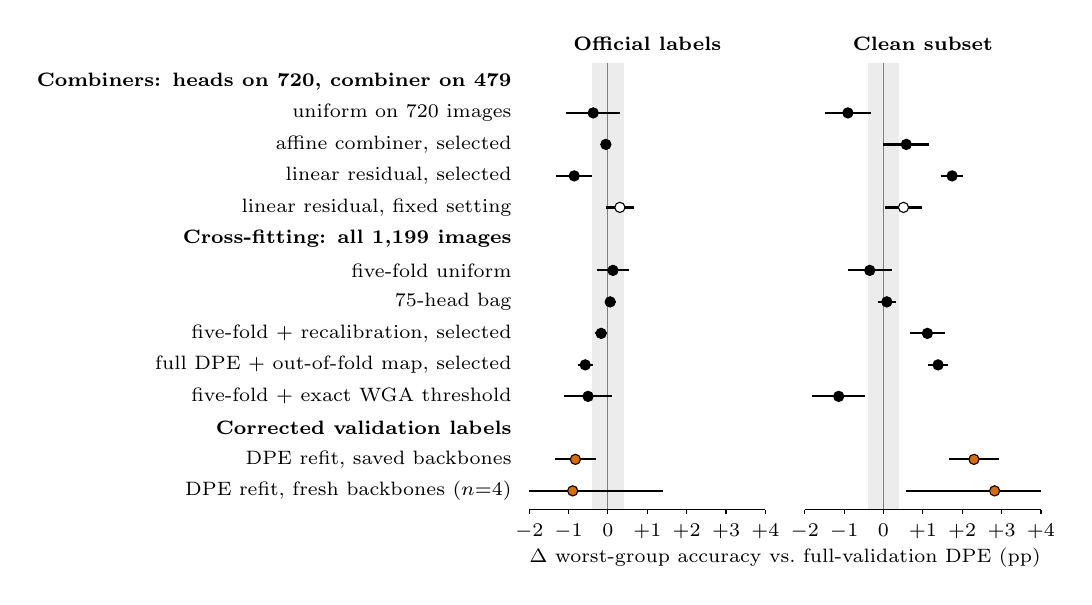
\begin{tikzpicture}[font=\scriptsize,y=0.40cm]
\fill[gray!15] (0.797,0.6) rectangle (1.203,-13.60);
\draw[gray] (1.000,0.6) -- (1.000,-13.60);
\draw (0.000,-13.60) -- (3.000,-13.60);
\draw (0.000,-13.60) -- ++(0,-0.15) node[below]{$-2$};
\draw (0.500,-13.60) -- ++(0,-0.15) node[below]{$-1$};
\draw (1.000,-13.60) -- ++(0,-0.15) node[below]{$0$};
\draw (1.500,-13.60) -- ++(0,-0.15) node[below]{$+1$};
\draw (2.000,-13.60) -- ++(0,-0.15) node[below]{$+2$};
\draw (2.500,-13.60) -- ++(0,-0.15) node[below]{$+3$};
\draw (3.000,-13.60) -- ++(0,-0.15) node[below]{$+4$};
\node[font=\scriptsize\bfseries] at (1.500,1.2) {Official labels};
\draw[thick] (0.469,-1) -- (1.157,-1);
\node[draw,circle,fill=black,inner sep=1.3pt] at (0.813,-1) {};
\draw[thick] (0.916,-2) -- (1.032,-2);
\node[draw,circle,fill=black,inner sep=1.3pt] at (0.974,-2) {};
\draw[thick] (0.339,-3) -- (0.804,-3);
\node[draw,circle,fill=black,inner sep=1.3pt] at (0.572,-3) {};
\draw[thick] (0.974,-4) -- (1.329,-4);
\node[draw,circle,fill=white,inner sep=1.3pt] at (1.152,-4) {};
\draw[thick] (0.860,-6) -- (1.267,-6);
\node[draw,circle,fill=black,inner sep=1.3pt] at (1.064,-6) {};
\draw[thick] (0.960,-7) -- (1.099,-7);
\node[draw,circle,fill=black,inner sep=1.3pt] at (1.029,-7) {};
\draw[thick] (0.836,-8) -- (0.992,-8);
\node[draw,circle,fill=black,inner sep=1.3pt] at (0.914,-8) {};
\draw[thick] (0.616,-9) -- (0.807,-9);
\node[draw,circle,fill=black,inner sep=1.3pt] at (0.712,-9) {};
\draw[thick] (0.443,-10) -- (1.053,-10);
\node[draw,circle,fill=black,inner sep=1.3pt] at (0.748,-10) {};
\draw[thick] (0.332,-12) -- (0.843,-12);
\node[draw,circle,fill=orange!85!black,inner sep=1.3pt] at (0.587,-12) {};
\draw[thick] (0.000,-13) -- (1.698,-13);
\node[draw,circle,fill=orange!85!black,inner sep=1.3pt] at (0.553,-13) {};
\fill[gray!15] (4.298,0.6) rectangle (4.703,-13.60);
\draw[gray] (4.500,0.6) -- (4.500,-13.60);
\draw (3.500,-13.60) -- (6.500,-13.60);
\draw (3.500,-13.60) -- ++(0,-0.15) node[below]{$-2$};
\draw (4.000,-13.60) -- ++(0,-0.15) node[below]{$-1$};
\draw (4.500,-13.60) -- ++(0,-0.15) node[below]{$0$};
\draw (5.000,-13.60) -- ++(0,-0.15) node[below]{$+1$};
\draw (5.500,-13.60) -- ++(0,-0.15) node[below]{$+2$};
\draw (6.000,-13.60) -- ++(0,-0.15) node[below]{$+3$};
\draw (6.500,-13.60) -- ++(0,-0.15) node[below]{$+4$};
\node[font=\scriptsize\bfseries] at (5.000,1.2) {Clean subset};
\draw[thick] (3.756,-1) -- (4.340,-1);
\node[draw,circle,fill=black,inner sep=1.3pt] at (4.048,-1) {};
\draw[thick] (4.495,-2) -- (5.082,-2);
\node[draw,circle,fill=black,inner sep=1.3pt] at (4.789,-2) {};
\draw[thick] (5.226,-3) -- (5.515,-3);
\node[draw,circle,fill=black,inner sep=1.3pt] at (5.371,-3) {};
\draw[thick] (4.517,-4) -- (4.991,-4);
\node[draw,circle,fill=white,inner sep=1.3pt] at (4.754,-4) {};
\draw[thick] (4.049,-6) -- (4.602,-6);
\node[draw,circle,fill=black,inner sep=1.3pt] at (4.325,-6) {};
\draw[thick] (4.424,-7) -- (4.659,-7);
\node[draw,circle,fill=black,inner sep=1.3pt] at (4.542,-7) {};
\draw[thick] (4.834,-8) -- (5.281,-8);
\node[draw,circle,fill=black,inner sep=1.3pt] at (5.057,-8) {};
\draw[thick] (5.063,-9) -- (5.323,-9);
\node[draw,circle,fill=black,inner sep=1.3pt] at (5.193,-9) {};
\draw[thick] (3.594,-10) -- (4.269,-10);
\node[draw,circle,fill=black,inner sep=1.3pt] at (3.931,-10) {};
\draw[thick] (5.327,-12) -- (5.970,-12);
\node[draw,circle,fill=orange!85!black,inner sep=1.3pt] at (5.649,-12) {};
\draw[thick] (4.788,-13) -- (6.500,-13);
\node[draw,circle,fill=orange!85!black,inner sep=1.3pt] at (5.911,-13) {};
\node[below] at (3.250,-14.50) {$\Delta$ worst-group accuracy vs.\ full-validation DPE (pp)};
\node[anchor=east,font=\scriptsize\bfseries] at (-0.1,0) {Combiners: heads on 720, combiner on 479};
\node[anchor=east] at (-0.1,-1) {uniform on 720 images};
\node[anchor=east] at (-0.1,-2) {affine combiner, selected};
\node[anchor=east] at (-0.1,-3) {linear residual, selected};
\node[anchor=east] at (-0.1,-4) {linear residual, fixed setting};
\node[anchor=east,font=\scriptsize\bfseries] at (-0.1,-5) {Cross-fitting: all 1,199 images};
\node[anchor=east] at (-0.1,-6) {five-fold uniform};
\node[anchor=east] at (-0.1,-7) {75-head bag};
\node[anchor=east] at (-0.1,-8) {five-fold + recalibration, selected};
\node[anchor=east] at (-0.1,-9) {full DPE + out-of-fold map, selected};
\node[anchor=east] at (-0.1,-10) {five-fold + exact WGA threshold};
\node[anchor=east,font=\scriptsize\bfseries] at (-0.1,-11) {Corrected validation labels};
\node[anchor=east] at (-0.1,-12) {DPE refit, saved backbones};
\node[anchor=east] at (-0.1,-13) {DPE refit, fresh backbones ($n{=}4$)};
\end{tikzpicture}
